% ─────────────────────────────────────────────────────────────────────────────
% Appendix B: Standalone Target-Network Results
% ─────────────────────────────────────────────────────────────────────────────
\section*{Appendix B: Standalone Target-Network Results}
\label{app:standalone}
This appendix presents the full method comparison on standalone target
networks --- configurations where a conventional MLP is trained directly via
gradient projection, without any hypernetwork wrapper or functional
regulariser. These results establish the baseline behaviour of each projection
method in its intended setting, prior to the hypernetwork integration examined
in the main text. All five benchmark streams are reported as per-task accuracy
trajectories in a single figure (Figure~\ref{fig:standalone_trajectories_all}):
Permuted-MNIST (5 tasks), Split-MNIST single-head (5 tasks), Split-MNIST
multi-head (5 tasks), Split-CIFAR10 (5 tasks), and Split-CIFAR100 (10 tasks).

% ── B.1  All benchmarks, single figure TRAJECTORIES ──────────────────────────
\begin{figure}[H]
    \centering
    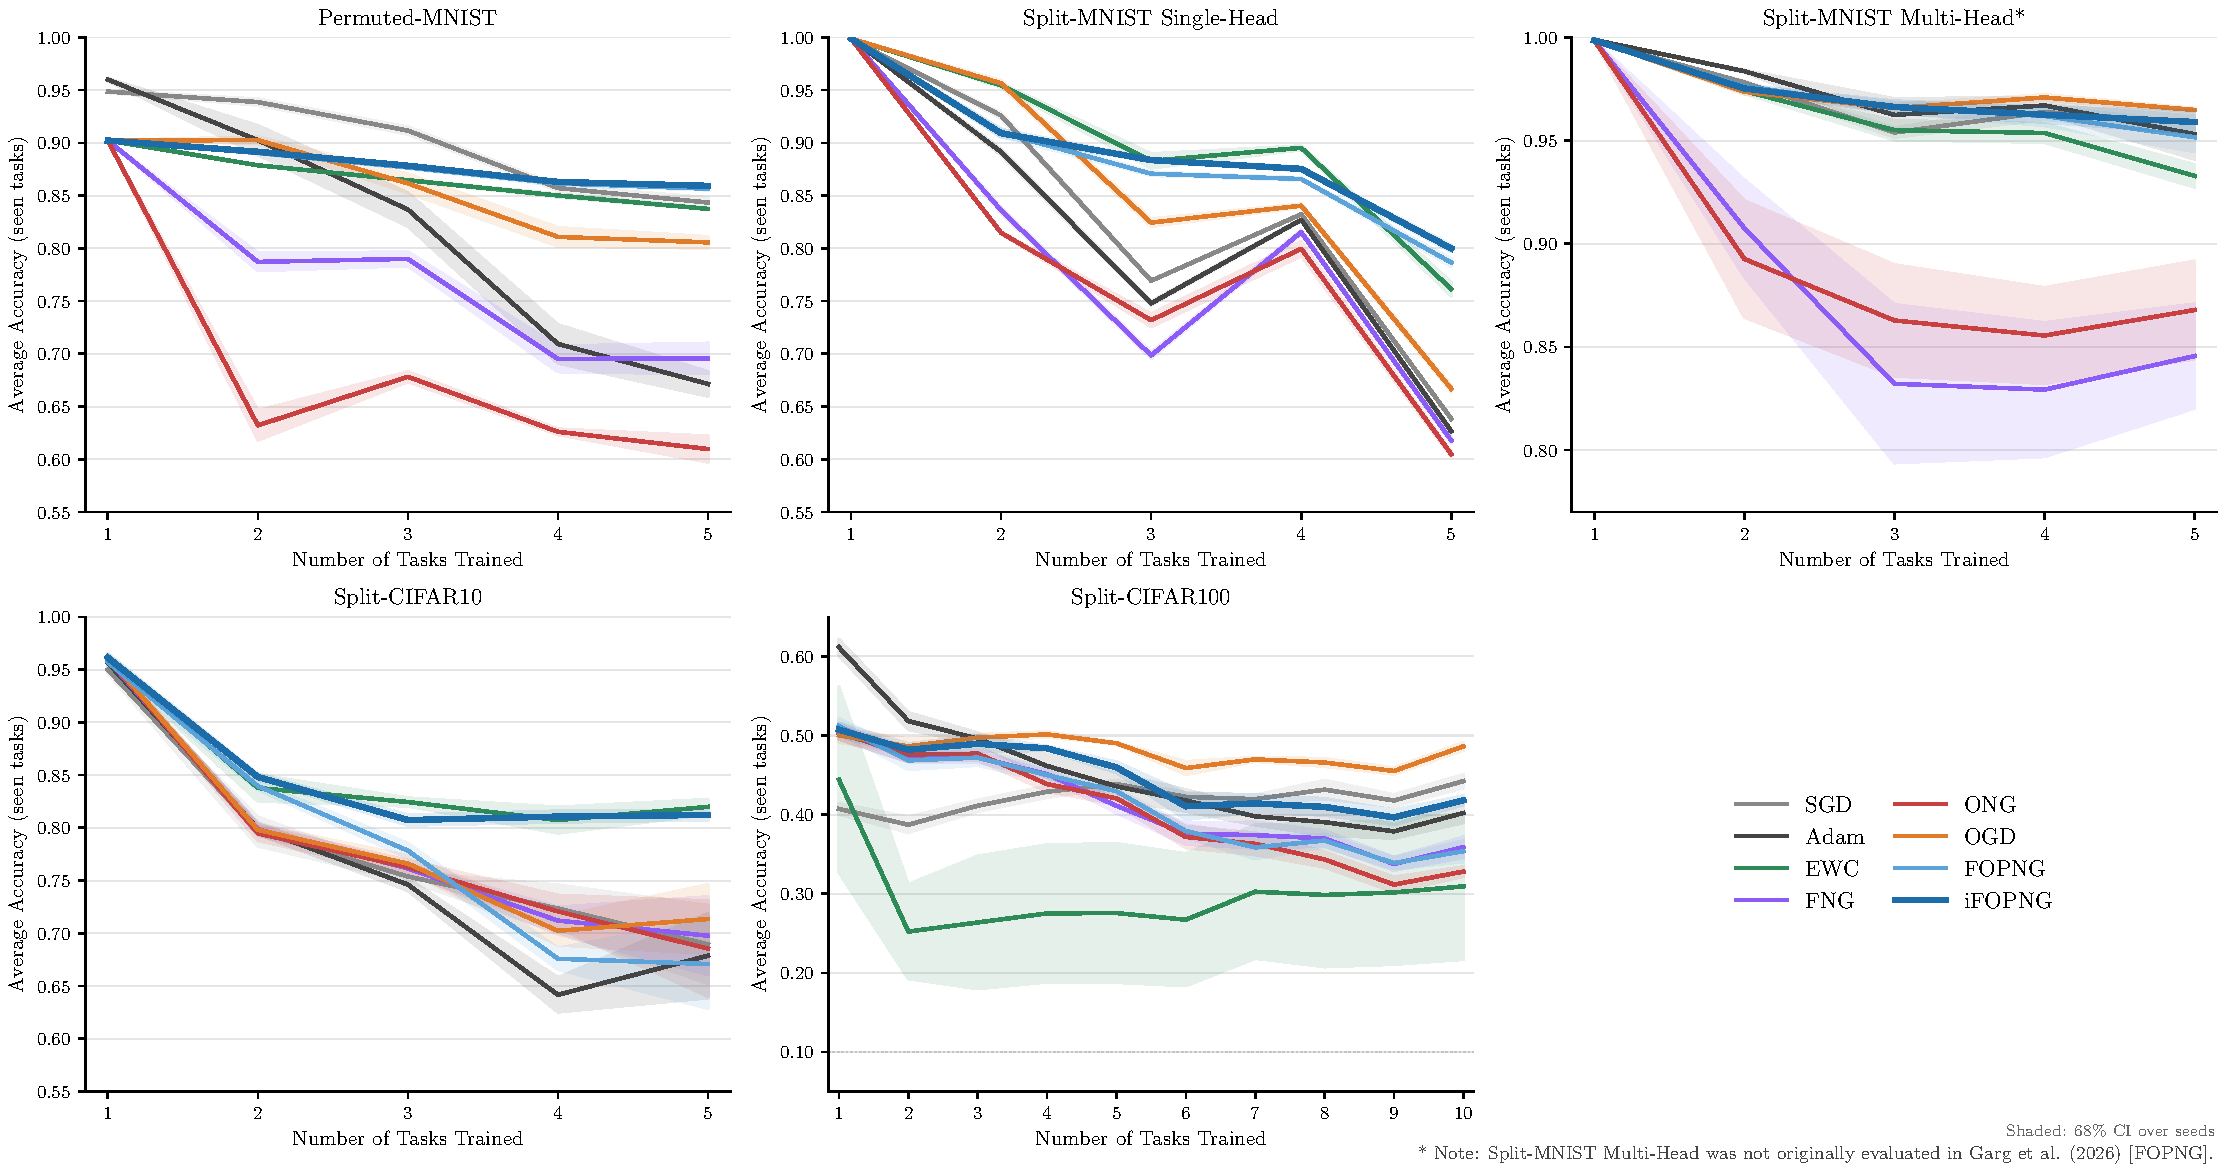
\includegraphics[width=\linewidth,height=0.82\textheight,keepaspectratio]{figures/garg-repl-grid.pdf}
    \caption{%
        \textbf{Standalone target-network accuracy trajectories across all
        benchmarks, replicating the evaluation protocol of
        \citet{garg_fisher-orthogonal_2026}.}
        Each panel is one benchmark: Permuted-MNIST (5T), Split-MNIST
        single-head (5T), Split-MNIST multi-head (5T), Split-CIFAR10 (5T), and
        Split-CIFAR100 (10T). Within each panel, the $x$-axis is the number of
        tasks trained so far and the $y$-axis is the average accuracy over all
        tasks seen up to that point. Lines show the seed mean for each method;
        shaded bands show the $68\%$ confidence interval over seeds. The
        trajectory format is used because the per-task curves are directly
        comparable to those reported by \citet{garg_fisher-orthogonal_2026},
        whose protocol this replicates. Backward-transfer (BWT) values quoted in
        the commentary below are reported summary statistics; this figure shows
        accuracy only.
    }
    \label{fig:standalone_trajectories_all}
\end{figure}

Per-benchmark commentary follows. All accuracies are seed means after the final
task, and BWT is the seed-mean backward transfer over the canonical five seeds.
%
\emph{Permuted-MNIST (5T).}
\texttt{iFOPNG} ($85.9\%$, BWT~$=-0.04$) and \texttt{FOPNG} ($85.7\%$,
BWT~$=-0.05$) trace the flattest trajectories, retaining near-peak accuracy
across all five tasks, with \texttt{SGD} ($84.3\%$) and \texttt{EWC} ($83.9\%$,
BWT~$=-0.03$) close behind. \texttt{OGD} ($80.6\%$, BWT~$=-0.18$) sits a step
lower. \texttt{FNG} ($69.6\%$), \texttt{Adam} ($67.1\%$), and \texttt{ONG}
($61.0\%$) decline steadily as tasks accumulate, with strongly negative BWT
($-0.31$, $-0.37$, $-0.44$ respectively), reflecting severe catastrophic
forgetting absent an effective projection or regularisation mechanism.
%
\emph{Split-MNIST SH (5T).}
\texttt{iFOPNG} maintains the highest trajectory throughout, ending at $80.0\%$
(BWT~$=-0.11$), with \texttt{FOPNG} close behind at $78.7\%$ (BWT~$=-0.14$) ---
confirming the Sub-RQ3 finding that the inertial combined-metric preconditioner
provides a consistent advantage under output-level interference. \texttt{EWC}
($76.1\%$) forms a second tier. \texttt{OGD} ($66.7\%$, BWT~$\approx-0.38$) is
far weaker than in the multi-head setting, reflecting the harder
gradient-subspace overlap of the shared head. The baselines \texttt{SGD}
($63.8\%$), \texttt{Adam} ($62.7\%$), \texttt{FNG} ($61.8\%$), and \texttt{ONG}
($60.5\%$) decline steeply across tasks (BWT~$\approx-0.42$ to $-0.48$).
%
\emph{Split-MNIST MH (5T).}
All trajectories remain near the ceiling, reflecting the low difficulty of the
binary per-task splits. \texttt{OGD}, \texttt{SGD}, \texttt{iFOPNG},
\texttt{Adam}, and \texttt{FOPNG} lead ($\approx 96.5$--$95\%$), with
\texttt{EWC} a short step below ($\approx 93\%$); \texttt{ONG} ($86.8\%$) and
\texttt{FNG} ($84.6\%$) are the exceptions, dipping over the sequence with
strongly negative BWT that indicates convergence instability rather than
gradual forgetting.
% VERIFY: ordering/heights of the MH leaders against the CSV.
%
\emph{Split-CIFAR10 (5T).}
\texttt{EWC} ($81.9\%$) and \texttt{iFOPNG} ($81.2\%$) lead with moderate
forgetting (BWT~$\approx-0.09$), tracing the highest trajectories. The remaining
methods fall to $67$--$71\%$ with substantially higher seed variance (wider CI
bands) and stronger decline. \texttt{FOPNG} is the weakest projection method at
$67.4\%$ --- a $13.8$~pp gap below \texttt{iFOPNG} that motivates the Sub-RQ3
comparison --- and \texttt{Adam} ($68.1\%$) performs comparably to the weaker
projection methods, confirming that the unconstrained baseline is not dominant
on harder standalone benchmarks.
%
\emph{Split-CIFAR100 (10T).}
\texttt{EWC} ($54.0\%$) traces the highest trajectory, followed by \texttt{OGD}
($49.0\%$) and \texttt{SGD} ($44.6\%$). \texttt{iFOPNG} ($42.9\%$) holds a
$6.0$~pp advantage over \texttt{FOPNG} ($36.9\%$), consistent with the Sub-RQ3
finding that parameter inertia provides increasing benefit as task count and
Fisher overlap grow. \texttt{Adam} ($40.4\%$) sits just behind \texttt{iFOPNG},
while \texttt{FNG} ($37.1\%$) closely mirrors \texttt{FOPNG}. \texttt{ONG}
declines fastest, ending lowest at $33.8\%$ (BWT~$\approx-0.38$). Random-chance
performance is $10\%$.
% CONFIRM: first-task init for CIFAR100 (Adam 1e-3 per protocol, not SGD 1e-2?).
% RESOLVE: EWC here = 54.0 but Table F.1 = 46.6 (lambda=10; table says lambda=50
%          collapsed/excluded). Contradiction — pick one lambda + one seed set.
% DISCLOSE/REVERT: EWC seed set (111 -> 314 substitution); verify lambda vs Garg Table 1.